\documentclass[a4paper,12pt]{article}
\usepackage[utf8]{inputenc}
\usepackage[T1]{fontenc}
\usepackage[slovene]{babel}
\usepackage{graphicx}
\usepackage{amssymb}
\usepackage{amsmath}
\usepackage{amsfonts}
\usepackage{amsthm}
\usepackage{lmodern}
\usepackage{float}
\usepackage{hyphenat} 
\usepackage[unicode]{hyperref}           
\graphicspath{{images/}}
\usepackage[colorinlistoftodos]{todonotes}

\theoremstyle{definition}

\newtheorem{defin}{Definicija}
\newtheorem{izrek}[defin]{Izrek}
\newtheorem{posl}[defin]{Posledica}
\newtheorem{trditev}[defin]{Trditev}

\begin{document}


\begin{titlepage}
	
	\center
		\textsc{\large Univerza v Ljubljani}\\
		\textsc{\large Fakulteta za matematiko in fiziko}\\	
		\textsc{\large Finančna matematika}\\[6cm]	
			
		\Large
		\textbf{Razbitje grafa z odstranjevanjem vozlišč in povezav}\\[1cm]
		\large
		\text{Projekt pri predmetu Finančni praktikum}\\[8cm] 
		\large 
		
		\large Avtorici:
		\textsc{Admira Abdić, Tia Krofel}\\	
		{\large Ljubljana, 6. december 2021}\\[1cm]
		
		\vfill
	
\end{titlepage}
	

\pagebreak

\section{Uvod}

\subsection{Opis problema}
V projektni nalogi si bomo podrobneje ogledali 
problem razbitja grafa z odstranjevanjem vozlišč in povezav. 
Za vhodni podatek bomo vzeli neusmerjen graf s podanima
vozliščema \emph{s} in \emph{t}.
Naloga projekta je nato pokazati, kako lahko izhodiščni graf 
razbijemo na več komponent, če smemo odstraniti največ eno vozlišče 
ter najmanjše možno število povezav, ob tem pa morata  
vozlišči \emph{s} in \emph{t} ležati v nepovezanih komponentah.

\subsection{Pristop k reševanju}
Najprej smo problem formulirali s pomočjo celoštevilskega linearnega programa,
nato pa s pomočjo implementiranih algoritmov za reševanje problema 
največjega pretoka in najmanjšega prereza v programskem jeziku Python
napisali še program, ki razbije podan graf na več komponent, tako da 
se podani vozlišči \emph{s} in \emph{t} ne nahajata v isti komponenti.
Na koncu smo generirali še nekaj neusmerjenih grafov različnih velikosti 
in na njih preizkusili delovanje našega programa.

\section{Celoštevilski linearni program}

Oglejmo si najprej, kako bi podan problem formulirali s celoštevilskim 
linearnim programom.

Izhajamo iz podanega neusmerjenega enostavnega grafa $G = (V, E)$ in 
uvedemo tri nove spremenljivke:

\begin{displaymath}
	x_{v} = \left\{
		\begin{array}{ll}
			1; &\text{v razbitem grafu vozlišče } v
			\text{ leži v isti komponenti kot vozlišče }s, \\
			0; &\text{sicer}.
		\end{array}\right.
\end{displaymath}

\begin{displaymath}
	y_{v} = \left\{
		\begin{array}{ll}
			1; &\text{vozlišče } v \text{ odstranimo iz grafa }G, \\
			0; &\text{sicer}.
		\end{array}\right.
\end{displaymath}

\begin{displaymath}
	z_{uv} = \left\{
		\begin{array}{ll}
			1; &\text{povezavo } uv \text{ odstranimo iz grafa }G, \\
			0; &\text{sicer}.
		\end{array}\right.
\end{displaymath}

Pri tem si vrednosti spremenljivke $x_v$ ogledamo za vsa vozlišča v grafu $G$, torej 
$\forall{v} \in V(G)$, vrednosti $y_v$ za vsa vozlišča izvzemši $s$ in $t$,
torej $\forall{v} \in V(G)\setminus \{s, t\}$, ki ju iz grafa $G$ ne želimo odstraniti, saj problem v tem primeru
ne bi imel smisla, kajti vedno bi lahko odstranili bodisi 
vozlišče $s$ bodisi vozlišče $t$ in s tem dosegli nepovezanost med $s$ in $t$.

Vrednosti $z_{uv}$ opazujemo pri vseh povezavah grafa $G$,
torej za $\forall uv \in E(G)$, a ker gre za neusmerjen graf, moramo preveriti 
povezanost v obeh smereh, kar pomeni, da za $\forall uv \in E(G)$ v množico povezav
dodamo še $vu$. Spodnjemu celoštevilskemu linearnemu programu torej podamo
bodisi usmerjen graf bodisi neusmerjen graf z razširjeno množico povezav, 
tj. $G' = (V, E'),$ kjer $E'$ za vsako povezavo $uv \in E$ vsebuje še $vu$.\\


Iščemo

$$ \min \sum_{uv \in E} z_{ij} $$

pri pogojih:

$$
\sum_{v \in V} y_{v} \le 1 
$$

$$
\forall uv \in E: x_u - x_v \le z_{uv} + y_v
$$

$$
x_s - x_t = 1 
$$

$$
\forall v \in V : y_v \in \{0,1\} 
$$

$$
\forall v \in V: x_v \in \{0,1\}
$$
 
$$
\forall uv \in E : z_{uv} \in \{0,1\}, z_{vu} \in \{0,1\} 
$$

Osrednji cilj programa je dobiti razbitje grafa $G= (V,E)$ z odstranitvijo 
največ enega vozlišča $v \in V$ in najmanjšega možnega števila povezav $(u,v) \in E$, 
tako da v razbitem grafu podani vozlišči $s \in V$ in $t \in V$ ne bosta več povezani.\\
\\
Pri tem smo upoštevali še druge pogoje. Pogoj $\forall uv \in E: x_u - x_v \le z_{u,v} + y_v $  zagotovi, 
da v primeru, ko je v prvotnem povezanem grafu obstajala povezava med vozliščema $u$ in $v$,
sedaj pa je vozlišče $u$ leži v isti komponenti kot vozlišče $s$, medtem ko vozlišče $v$ z $s$ ni povezano, 
smo morali odstraniti bodisi povezavo med njima bodisi vozlišče $v$.\\

Končno mora biti izpolnjen še pogoj $ x_s - x_t = 1$, 
ki predstavlja nepovezanost vozlišča $t$ z vozliščem $s$ v razbitem grafu. \\


\section{Problem največjega pretoka in najmanjšega prereza}

\subsection{Teoretično ozadje}


Naj bo $G = (V, E)$ graf, kjer $V = V(G)$ predstavlja množico vozlišč,
$E = E(G)$ pa množico povezav grafa $G$.\newline

Najprej si oglejmo različne načine razbitja posameznega grafa.


Množica $S \subseteq V(G)$ je \textit{točkovni prerez} na grafu G,
če ima graf $G - S$ več komponent kot $G$. \textit{Povezanost po točkah}
grafa $G$ je enaka minimalni moči množice $S$, za katero je $G - S$ 
nepovezan (ali ima le eno točko). Graf je $k$-povezan po točkah, 
če je njegova povezanost po točkah vsaj $k$.

Množico $F \subseteq E(G)$ pa imenujemo \textit{razdelitvena množica 
povezav} na grafu $G$, če ima graf $G - F$ več komponent kot $G$.
\textit{Povezanost po povezavah} grafa $G$ je enaka minimalni moči
množice $F$, za katero je $G - F$ nepovezan. Graf je $k$-povezan po
povezavah, če je njegova povezanost po povezavah vsaj $k$. \newline


Ker nas bo zanimalo tudi, kako lahko dan problem rešimo s pomočjo
algoritmov za reševanje problema največjega pretoka, definiramo še 
slednjega. \\


\textbf{Problem največjega pretoka}: Naj bo $G = (V, E)$ usmerjen graf,
$s \in V$ (izvor) in $t \in V$ (ponor) dani odlikovani vozlišči,
število $c_{ij} \geq 0$ pa naj za vsako povezavo $(i, j) \in E$ 
predstavlja prepustnost povezave $(i, j)$.
Prepustnost lahko na vse pare razširimo na sledeč način:
\begin{displaymath}
	c(i,j) = \left\{
		\begin{array}{ll}
			c_{ij}, &\text{če } (i,j) \in E, \\
			0, &\text{če } (i, j) \notin E.
		\end{array}\right.
\end{displaymath}
Urejeno četverko $(G, s, t, c)$ imenujemo \textit{(pretočno) omrežje}.
Na podlagi teh podatkov nato iščemo največji pretok $f$ v 
pretočnem omrežju $(G, s, t, c).$ \\

Za preslikavo $f: V \times V \to \mathbb{R}$ velja, da je pretok v omrežju $(G,s,t,c)$, 
če zadošča naslednjim pogojem:\\
\begin{enumerate}
	\item $f(i,j) \geq c(i,j)$ za vse $i, j \in V$ (ustreznost pretoka),
	\item $f(i,j) = - f(i,j)$ za vse $i,j \in V$ (antisimetričnost pretoka),
	\item $\sum_{i \in V} f(i,j) = 0 $ za vse $i, j \in V \setminus {s,t}$ (Kirchhoffovi zakoni).\\
\end{enumerate}
Število $f(A,B) = \sum_{i \in V} f(i,j)$ potem imenujemo velikost pretoka $f$.\\


Pri \textbf{problemu najmanjšega prereza} imamo prav tako podano
pretočno omrežje $(G, s, t, c)$ in iščemo prerez z najmanjšo prepustnostjo.

Ob tem kot prerez omrežja $(G,s,t,c)$ razumemo par množic $A,B \subseteq V$, kjer je:
$A \cup B = V $, $A \cap B = \emptyset$ in $s \in A, t \in B$.\\
\newline
\newline
In končno si oglejmo še \textbf{Ford-Fulkersonov izrek, KID}:\\
Za vsak pretok $f$ v omrežju $(G,s,t,c)$ so naslednje tri trditve enakovredne:
\begin{enumerate}
	\item $f$ je največji pretok v $(G,s,t,c)$,
	\item v $(G,s,t,c)$ ni povečujočih poti za $f$,
	\item v $(G,s,t,c)$ obstaja prerez (A,B), tako da je $ \lvert f \rvert = c(A,B)$.
\end{enumerate}
 

\subsection{Uporaba algoritmov za reševanje našega problema}

Na podlagi zgornje teorije si sedaj poglejmo, kako si lahko z implementiranimi
algoritmi za iskanje največjega pretoka in najmanjšega prereza pomagamo pri 
reševanju našega problema.\\

Znotraj programskega okolja Python bomo uporabili knjižnico \emph{NetworkX}, ki je namenjena
analizi kompleksnih omrežij in ima že implementirane funkcije za iskanje 
največjega pretoka in najmanjšega prereza v omrežju. Na koncu bomo za prikaz 
naših generiranih grafov uporabili še knjižnico \emph{mathplotlib},
pri samem generiranju grafov pa si bomo pomagali s funkcijami iz knjižnice \emph{random}.\\

S predpostavko, da bomo našemu programu podali neusmerjen graf $G = (V,E)$, 
bo naš algoritem na začetku preko funkcije \textit{G.to\_directed()}
za vsako $uv \in E$ povezavo v množico $E$ dodal še povezavo $vu$ in 
nov graf obravnaval kot usmerjenega.

Nato bomo preverili, če vozlišči $s$ in $t$ v podanem grafu 
slučajno nista povezani - v tem primeru lahko zaključimo, saj smo dosegli naš cilj.

Nato si bo ogledal, ali je slučajno možno prekiniti povezavo med $s$ in $t$ 
že z odstranitvijo enega samega vozlišča (ki ni ne $s$ ne $t$). 
V tem primeru bo problem rešen in po tem, ko bomo odstranili vozlišče,
nam ne bo treba odstraniti nobene dodatne povezave.

Če pa željeno razbitje grafa ne bo mogoče z odstranitvijo enega samega vozlišča,
si bomo ogledali, kakšen je največji pretok v pretočnem omrežju, ki ga iz podanega
grafa (transformiranega v usmerjenega) dobimo tako, da za vsako povezavo določimo 
še pretočnost, tj. \textit{capacity}. Mi bomo to storili na generiranih grafih 
že na začetku, in sicer bo pretočnost vsake izmed naših povezav enaka 1, 
s čimer si že na začetku zagotovimo,
da je največji pretok na tem omrežju enak najmanjšemu številu povezav, ki jih moramo
odstraniti za to, da prekinemo povezanost med $s$ in $t$.

Dobljen največji pretok v celotnem grafu bomo primerjali z največjimi pretoki podgrafov,
ki jih bomo dobili tako, da bomo naenkrat iz podanega grafa odstranili po eno vozlišče.
Ker si želimo odstraniti najmanjše možno število povezav, bomo med njimi poiskali tistega,
ki ima najmanjšo vrednost največjega pretoka.

Nato bomo prvotni neusmerjeni graf, vozlišči $s$ in $t$ ter vozlišče (oziroma vozlišča), 
ki se ga najbolj splača odstraniti, poslali funkciji \textit{razbij}, ki bo poskrbela
za ustrezno razbitje grafa z odstranitvijo najmanjšega možnega števila povezav, potem pa
bo naš algoritem narisal še razbit graf.

\subsection{Preizkus algoritma}

Na koncu s pomočjo matrik generirajmo še nekaj grafov.
V naši matriki bo enica na mestu [$i$][$j$] pomenila, da sta vozlišči $i$ in $j$
v grafu povezani, ničla pa, da nista.

Ker generiramo neusmerjene grafe, bodo matrike simetrične, in ker ne želimo,
da bi naši grafi vsebovali zanke, zadošča, da s pomočjo knjižnice $random$ 
naključno z ničlami in enicami zapolnimo le tisti del matrike, ki se nahaja
strogo nad diagonalo. 
Če funkciji \textit{matrika\_povezav} ne podamo nobenega argumenta, 
bo imela pet vrstic in pet stolpcev,
drugače pa lahko njeno velikost določimo sami. 

Nato s funkcijo \textit{matrika\_v\_neusmerjen\_graf(matrika)} generiramo
neusmerjen graf, ki ima povezave med tistimi vozlišči, kjer se v matriki 
nahaja enica (ker vozlišča označimo s številkami, to pomeni, da če $v1 < v2$,
potem sta $v1$ in $v2$ povezani, če bo v matriki na mestu, ki ustreza 
vrstici $v1$ in stolpcu $v2$, enica).

Zatem si zopet pomagamo s knjižnico $random$ in izmed vozlišč v našem generiranem grafu
naključno izberemo $s$ in $t$. Takšen graf nato narišemo, potem pa ga pošljemo v
zgoraj opisan algoritem skupaj z izbranima vozliščema $s$ in $t$.

\subsection{Rezultati}

Če poženemo \textit{algoritem.py}, kjer je zapisana tudi vsa zgoraj opisana koda,
dobimo na primer naslednji rezultat (slike se nam odpirajo v dodatnem oknu in šele po
ogledu ter zaprtju prikaza posameznega grafa se bo izpisovanje v terminalu nadaljevalo):

\begin{figure}[H]
	\caption{Prvi poskus, prvotni graf}
	\centering
	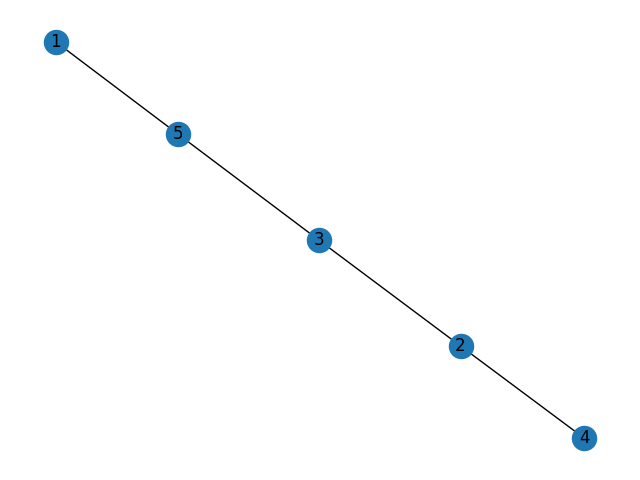
\includegraphics[scale=0.4]{slikovni_prikaz/Figure_1_0}
\end{figure}

V terminalu nam program sporoči, da gre tukaj za neusmerjen graf, 
z množico vozlišč $V = \{1, 5, 2, 3, 4\}$ in množico povezav $E = \{(1, 5), (5, 3), (2, 3), (2, 4)\}$.
Za izbrani vozlišči sta naključno izbrani $s = 4$ in $t = 3$. 
Prav tako nam program pove, da je podan graf je brez odstranjenih vozlišč
glede na povezanost med $s$ in $t$ 1-povezan po povezavah.

\begin{figure}[H]
	\caption{Prvi poskus, razbit graf}
	\centering
	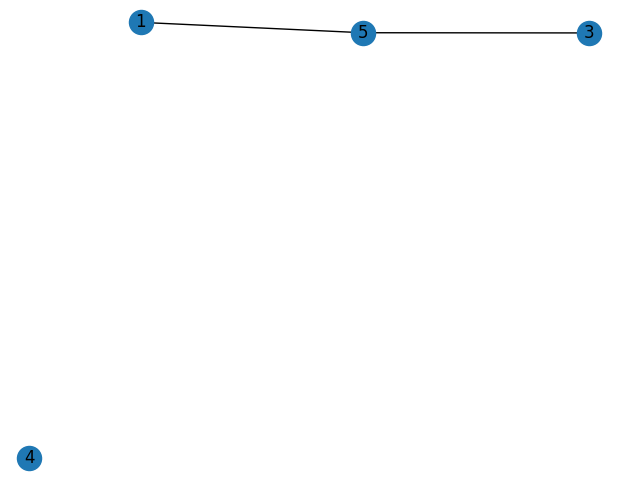
\includegraphics[scale=0.4]{slikovni_prikaz/Figure_1_1}
\end{figure}

Nato nam algoritem v terminal izpiše, da je prvotni graf lahko uspešno razbit z 
odstranitvijo vozlišča 2 in ohranjenimi vsemi povezavami,
torej vrne neusmerjen graf z vozlišči $V' = \{1, 5, 3, 4\}$ in povezavami $E' = \{(1, 5), (5, 3)\}$.\\

Oglejmo si še primer programa, ki mu za velikost matrike podamo $10$:

\begin{figure}[H]
	\caption{Drugi poskus, prvotni graf}
	\centering
	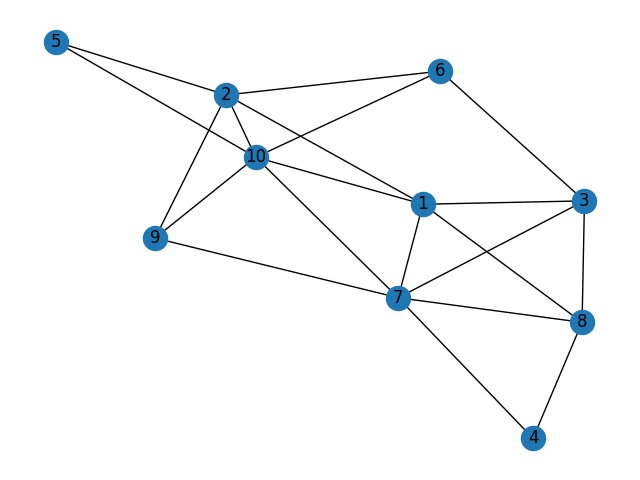
\includegraphics[scale=0.4]{slikovni_prikaz/Figure_2_0}
\end{figure}

V terminalu nam program sporoči, da gre tukaj za neusmerjen graf, 
z množico vozlišč $V = \{1, 2, 3, 7, 8, 10, 5, 6, 9, 4\}$ in množico povezav 
$E =$ \{(1, 2), (1, 3), (1, 7), (1, 8), (1, 10), (2, 5), (2, 6), (2, 9), (2, 10), (3, 6), (3, 7), (3, 8), (7, 4), (7, 8), (7, 9), (7, 10), (8, 4), (10, 5), (10, 6), (10, 9)\}.
Za izbrani vozlišči sta naključno izbrani $s = 9$ in $t = 3$. 
Prav tako nam program pove, da je podan graf je brez odstranjenih vozlišč
glede na povezanost med $s$ in $t$ 3-povezan po povezavah.

Nato ugotovi, da razbitje tega grafa z odstranitvijo le enega vozlišča
ni mogoče in da je najmanjse stevilo povezav, ki jih moramo odstraniti, 2, 
do tega pa lahko pridemo na vec različnih načinov, in sicer z odstranitvijo enega
izmed vozlišč $2, 7$ ali $10$.

\begin{figure}[H]
	\caption{Drugi poskus, razbit graf z odstranjenim vozliščem 2}
	\centering
	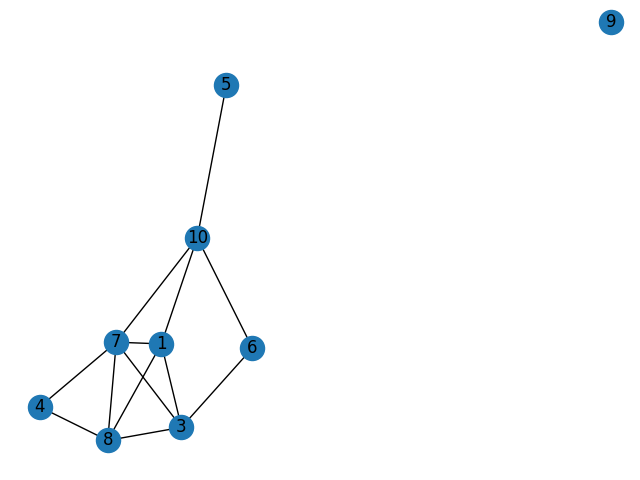
\includegraphics[scale=0.4]{slikovni_prikaz/Figure_2_1}
\end{figure}

Če odstranimo vozlišče $2$, je graf, ki ga sedaj razbijamo, glede na $s$ in $t$ 
$2$-povezan po povezavah in zato odstranimo še povezavi $(9, 7)$ in $(9, 10)$
ter dobimo razbit neusmerjen graf z vozlišči $V' = \{1, 3, 7, 8, 10, 5, 6, 9, 4\}$ in povezavami 
$E' =$ \{(1, 3), (1, 7), (1, 8), (1, 10), (3, 6), (3, 7), (3, 8), (7, 4), (7, 8), (7, 10), (8, 4), (10, 5), (10, 6)\}.\\

\begin{figure}[H]
	\caption{Drugi poskus, razbit graf z odstranjenim vozliščem 7}
	\centering
	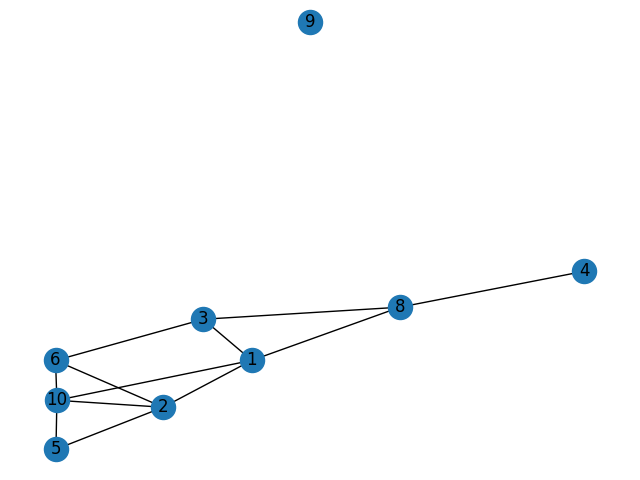
\includegraphics[scale=0.4]{slikovni_prikaz/Figure_2_2}
\end{figure}

Če odstranimo vozlišče $7$, je graf, ki ga sedaj razbijamo, glede na $s$ in $t$ 
$2$-povezan po povezavah in zato odstranimo še povezavi $(9, 2)$ in $(9, 10)$
ter dobimo razbit neusmerjen graf z vozlišči $V' = \{1, 2, 3, 8, 10, 5, 6, 9, 4\}$ in povezavami 
$E' =$ \{(1, 2), (1, 3), (1, 8), (1, 10), (2, 5), (2, 6), (2, 10), (3, 6), (3, 8), (8, 4), (10, 5), (10, 6)\}.\\

\begin{figure}[H]
	\caption{Drugi poskus, razbit graf z odstranjenim vozliščem 10}
	\centering
	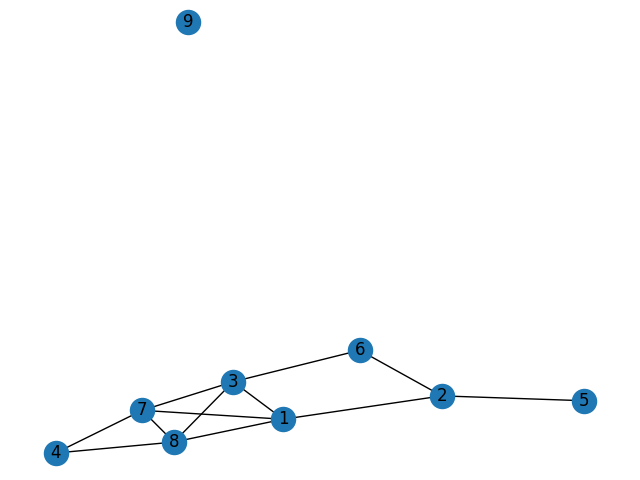
\includegraphics[scale=0.4]{slikovni_prikaz/Figure_2_3}
\end{figure}

Če odstranimo vozlišče $10$, je graf, ki ga sedaj razbijamo, glede na $s$ in $t$ 
$2$-povezan po povezavah in zato odstranimo še povezavi $(9, 2)$ in $(9, 7)$
ter dobimo razbit neusmerjen graf z vozlišči $V' = \{1, 2, 3, 7, 8, 5, 6, 9, 4\}$ in povezavami 
$E' =$ \{(1, 2), (1, 3), (1, 7), (1, 8), (2, 5), (2, 6), (3, 6), (3, 7), (3, 8), (7, 4), (7, 8), (8, 4)\}.\\

\subsection{Opažanje}

Po večkratnem eksperimentiranju s spreminjanjem velikosti matrike in ponavljanjem poskusa
ob isti velikosti matrike lahko ugotovimo, da je ob večanju matrik (in s tem tudi števila 
vozlišč v grafih) vedno manj možnosti, da bo razbitje grafa možno že z odstranitvijo
enega samega vozlišča, imeli pa bomo vedno več različnih opcij, katero vozlišče naj odstranimo,
da bomo morali zatem odstraniti najmanjše možno število povezav, ki bo pri vseh teh vozliščih
enako.

\section{Viri}
\begin{itemize}
	\item M. Petkovšek, Material pri predmetu Optimizacijske strukture, 2020.
	\item Dokumentacija knjižnice NetworkX, dostopna na naslovu: \url{https://networkx.org/documentation/stable/index.html},
			dostopano dne 27. 11. 2021.
\end{itemize}

\end{document}